\documentclass[IB]{TFUOC}%IB: CASTELLANO, CAT: CATALÁN, ENG: ANGLÈS

\usepackage[numbers]{natbib}

%Introducción de datos del trabajo
\title{Modelado estilístico de la novela de misterio - Un análisis computacional de autores canónicos}
\titcrt{\textit{Whodunit} estilométrico} %Título corto que aparecerá a la cabecera
\author{Teresa García Ceva}
\date{15 de junio de 2026}


\nomPDC{Jonatan Martín Rodríguez}
\nomPRA{Nombre Profesorado Responsable}
\titulac{Grado en Ciencia de datos aplicada}
\area{Área del trabajo}
\idioma{Castellano}
\credits{15}
\parcla{palabra, clave, trabajo}

\licenc{ccBy}
%Posibles licencias
%ccByNcNd
%ccByNcSa
%ccByNc
%ccByNd
%ccBySa
%ccBy
%GNU
%copyright


%%%%%%%%%%
% Resumen en el idioma

\abstractidioma{
Máximo 250 palabras, con la finalidad, contexto de aplicación, metodología, resultados y conclusiones del trabajo.
}

% Resumen en inglés.
\abstractenglish{
A maximum of 250 words, detailing the purpose, contexto of application, methodology, results and conclusiones of the work.
}

\begin{document}

\estructura

\tableofcontents

\listoffigures

\listoftables


\chapter{Introducción}

Esta plantilla se concibe como una guía para el estudiante. Se puede adaptar a las necesidades de cada trabajo, siempre que el/la tutor/a del trabajo esté de acuerdo.

\section{Contexto y justificación del trabajo}

Punto de partida del trabajo (¿Cuál es la necesidad a cubrir? ¿Por qué es un tema relevante? ¿Cómo se resuelve el problema de momento?) y aportación realizada (¿Qué resultado se quiere obtener?).\cite{konect:2017:moreno_crime}

Es importante tener en cuenta que el trabajo final tiene que ser comprensible para cualquier persona que conozca el área de conocimiento, pero no tiene porque ser experta en el tema del que versa el trabajo.

\section{Objetivos del trabajo}

Listado de los objetivos del trabajo.

\section{Impacto en sostenibilidad, ético-social y de diversidad}
\label{s:etic}

Esta sección tendría que identificar los impactos positivos y/o negativos del trabajo final en las tres dimensiones de la competencia transversal UOC “Compromiso ético y global”.

La Guía transversal sobre la Competencia Ética y Global os ayudará a redactar estos apartados.

\section{Preguntas de investigación e hipótesis de trabajo}
\section{Alcance, supuestos y limitaciones iniciales}
\section{Impacto en sostenibilidad, ético-social y de diversidad}
\section{Enfoque y método seguido}

Mención de cuáles son las posibles estrategias para llevar a cabo el trabajo y cuál es la estrategia elegida (desarrollar un producto nuevo, adaptar un producto existente...). Hay que incluir una valoración de por qué esta es la estrategia más apropiada para conseguir los objetivos.

\section{Planificación del trabajo}

Descripción de los recursos necesarios para hacer el trabajo, las tareas a realizar y una planificación temporal de cada tarea mediante un diagrama de Gantt o similar. Esta planificación tendría que marcar cuáles son los hitos parciales de cada una de las PEC.

Identificación de los posibles riesgos que pueden hacer que esta planificación no se cumpla y descripción de los planes de mitigación o alternativos en caso de que estos riesgos sean un problema.

\section{Breve sumario de productos obtenidos}

No hay que entrar en detalle: la descripción detallada se hará en el resto de capítulos.

\section{Estructura de la memoria}

Breve explicación de los contenidos de cada capítulo y su relación con el proyecto global.

\chapter{Marco teórico y estado del arte}

\section{Estilometría y atribución de autoría: conceptos clave}
\section{Métodos clásicos de estilometría}
\section{Enfoques modernos en atribución de autoría}
\section{Evaluación en atribución de autoría}
\section{Explicabilidad e interpretabilidad en PLN}
\section{Herramientas y trabajos de referencia}

%Estado del arte del tema en cuestión. Tendría que acabar mostrando por qué el trabajo es importante y aporta algo, y con las hipótesis del trabajo.

\chapter{Datos: construcción del corpus y gestión de la información}

\section{Fuentes y criterios de selección/exclusión}
\section{Metadatos y normalización}
\section{Calidad del texto y control de artefactos}
\section{Análisis exploratorio del corpus}
\section{Marco ético y legal del corpus}
\section{Plan de gestión de datos y reproducibilidad}

\chapter{Materiales y métodos}

\section{Entorno y herramientas}
\section{Diseño experimental}
\section{Preprocesamiento}
\section{Extracción de rasgos clásicos}
\section{Representaciones distribuidas}
\section{Modelos de clasificación}
\section{Ajuste y validación}
\section{Explicabilidad del sistema}
\section{Implementación del pipeline/herramienta}


\chapter{Resultados}

\section{Descripción final del corpus}
\section{Rendimiento de modelos}
\section{Comparativa: enfoques clásicos vs. modernos}
\section{Interpretabilidad global}
\section{Interpretabilidad local y análisis de casos}
\section{Robustez y validez}

Detallad en este apartado los resultados obtenidos utilizando la metodología descrita en el apartado anterior.

Las figuras tienen que estar explicadas y citadas en el texto, como la \ref{fig:my_label}, en la cual se muestra el error en función de la distancia, en unidades arbitrarias. En todas las gráficas tiene que haber el título de los ejes.

\begin{figure}[!htbp]
    \centering
    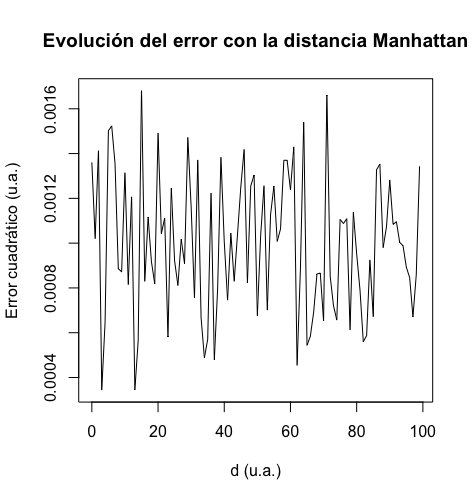
\includegraphics[width=7truecm]{Rplotmanh.png}
    \caption{Error en función de la distancia en unidades arbitrarias.}
    \label{fig:my_label}
\end{figure}

\chapter{Discusión y conclusiones}

\section{Discusión de hallazgos}

Discusión de los resultados en el contexto del proyecto. Es en este apartado donde cobran sentido y en el cual se responden las preguntas de investigación y se muestra como los resultados dan respuesta a los problemas planteados.

\section{Limitaciones}

\section{Implicaciones sociotécnicas}

\section{Conclusiones finales}

Este capítulo tiene que incluir:
\begin{itemize}
	\item Una descripción de las conclusiones del trabajo:
	\begin{itemize}
    	\item Una vez se han obtenido los resultados, ¿qué conclusiones se extraen?
    	\item ¿Estos resultados son los esperados? ¿O han sido sorprendentes? ¿Por qué?
	\end{itemize}
	\item Una reflexión crítica sobre el logro de los objetivos planteados inicialmente:
	\begin{itemize}
    	\item ¿Hemos logrado todos los objetivos? Si la respuesta es negativa, ¿por qué motivo?
	\end{itemize}
	\item Un análisis crítico del seguimiento de la planificación y metodología a lo largo del producto:
	\begin{itemize}
    	\item ¿Se ha seguido la planificación?
    	\item ¿La metodología prevista ha sido suficientemente adecuada?
    	\item ¿Ha habido que introducir cambios para garantizar el éxito del trabajo? ¿Por qué?
	\end{itemize}
	\item De los impactos previstos en \ref{s:etic}, ético-sociales, de sostenibilidad y de diversidad, evaluar/mencionar si se han mitigado (si eran negativos) o si se han conseguido (si eran positivos).
	\item Si han aparecido impactos no previstos a \ref{s:etic}, evaluar/mencionar cómo se han mitigado (si eran negativos) o que han aportado (si eran positivos).
	\item Las líneas de trabajo futuro que no se han podido explorar en este trabajo y han quedado pendientes.
	\item Una descripción de las conclusiones del trabajo: Qué lecciones se han aprendido del trabajo?
	\item Una reflexión crítica sobre el logro de los objetivos planteados inicialmente: Hemos conseguido todos los objetivos? Si la respuesta es negativa, por qué motivo?
	\item De los impactos previstos a la sección \ref{s:etic}, una evaluación, o al menos, mención, sobre si se han mitigado (si eran negativos) o si se han conseguido (si eran positivos).
\end{itemize}

\section{Trabajos futuros}

Las líneas de trabajo futuro que no se han podido explorar en este trabajo y han quedado pendientes.

\section{Seguimiento de la planificación}

Un análisis crítico del seguimiento de la planificación y metodología a lo largo del trabajo:
\begin{itemize}
    \item  Se ha seguido la planificación?
    \item La metodología prevista ha sido la adecuada?
    \item Ha habido que introducir cambios para garantizar el éxito del trabajo? ¿Por qué?
\end{itemize}

\chapter{Glosario}

Definición de los términos y acrónimos más relevantes utilizados dentro de la Memoria.


\chapter{Apéndices}

Listado de apartados que son demasiado extensos para incluir dentro de la memoria y tienen un carácter autocontenido (por ejemplo, manuales de usuario, manuales de instalación, etc.)

Dependiendo del tipo de trabajo, es posible que no haya que añadir algún anexo.

\bibliographystyle{apalike-es}
\bibliography{bibliography.bib}
\addcontentsline{toc}{chapter}{Bibliografía}

\end{document}
